\documentclass{scrreprt}
\usepackage[english]{babel}
\usepackage[T1]{fontenc}
\usepackage{lmodern}
\usepackage{blindtext}
\usepackage[utf8]{inputenc}
\usepackage{siunitx} %For unit handling%
\renewcommand{\familydefault}{\sfdefault}
\newcommand{\unit}[1]{\ensuremath{\, \mathrm{#1}}}
\usepackage{amssymb, amsmath, cancel, ulem, graphicx, float, tabularx, multirow, bm}
\usepackage{amsmath}
\usepackage{caption}
\usepackage{subcaption}
\usepackage{mathtools}
\usepackage{tikz}
\usepackage{commath}
\usepackage{nameref}
\newcommand*\circled[1]{\tikz[baseline=(char.base)]{
            \node[shape=circle,draw,inner sep=1pt] (char) {#1};}}
\renewcommand{\phi}{\varphi}


\setcounter{secnumdepth}{5}
\setcounter{tocdepth}{5}

\author{Urs Gerber\\09-921-156 \and Gian-Luca Mateo\\11-113-545}
\date{2nd of May 2013}

\title{Spinning Top}
\subtitle{Practical course report}

\begin{document}

\maketitle

\tableofcontents
\newpage

\chapter{Experiment: Spinning Top}

\section{Introduction}

\subsection{Goal of the experiment}
The goal of this experiment is to analize and measure the properties of a spinning top. More precisely, we are first and foremost interested in the top's precession period when applying variable momenta at different angular frequencies.
 
\subsection{Theory}
A top consists of a rigid body which is free to rotate around a fixed point $0$. Generally said, the motion is a rotation around a momentary rotation axis with an arbitrary orientation. In this experiment, however, we use a much simpler variation of the general top, called a rotationally symmetric top, which makes the equations of motion much simpler.\\

In the experiment we investigate the behavior of a very fast spinning top under the influence of a torsional moment caused by gravity. Thereto a massive metal disk is linked to an electric motor via a shaft. Said shaft is hinged at its center of gravity so that no forces are applied in resting state. On the side where the motor is mounted, a weight can be attached to exert torque on the shaft and consequently the axis of rotation of the top which results in a precession motion.\\

\paragraph*{Precession period $T_P$}
From the equation of motion for the rotation of a rigid body 

\begin{equation}
\vec{M} = \frac{\dif \vec{L}}{\dif t}
\end{equation}

and

\begin{equation}
\vec{L} = J \cdot \vec{\omega}
\end{equation}

where $\vec{M}$ is the applied torsional moment, $\vec{L}$ the angular momentum, $J$ the body's moment of inertia and $\omega$ the angular velocity, one can show that the body's precession frequency is described by:

\begin{equation}
\Omega_P = \frac{|\vec{M}|}{|\vec{L}\cdot \sin \vartheta|}
\end{equation}

If we insert the moment of the weight attached to the shaft $\vec{M} = \vec{l} \times \vec{G} \Rightarrow M = m g \cdot l \cdot \sin \vartheta$ we get

\begin{equation}
\Omega_P = \frac{mg\cdot l}{J\cdot \omega}
\end{equation}
and therefore a procession period of
\begin{equation}
T_P = \frac{2\pi}{\Omega_P} = \frac{2\pi J \omega_0}{mgl}
\end{equation}

\subsubsection{Moment of Inertia}

We find the moment of inertia $J$ of the top's spinning disk by dropping a weight with mass $m$ attached to the disk via a thread from a height $h$ and measuring the resulting angular frequency $\omega_0$. Using simple energy conservation laws, we get

\begin{equation}
\label{eq:inertia}
J = \frac{2mgh}{\omega_0^2} - m R^2
\end{equation}

as proven in section ''\nameref{sec:preliminary_exercises}``

\subsubsection{Parenthesis: Preliminary Exercises}
\label{sec:preliminary_exercises}


\subsubsection{Error analysis}
\paragraph*{Moment of Inertia}

\begin{equation}
s_J^2 = 4 m^2 \left( r^2 s_r^2 + \frac{4 g^2 h^2 s_w^2}{\omega^6} \right)
\end{equation}

\section{Experiment setup and execution}

\subsection{Used materials}
The materials used in this experiment are the following:
\begin{itemize}
\item A rotationally symmetric top, hinged and turnable in the z-axis
\item An electric engine, attached to the top
\item A piece of string, about $1 \unit{m}$ in length, attachable to the metal disk of the top, with a hook to attach weights
\item Four weights, $0.2 \unit{kg}$, $0.46 \unit{kg}$, $1 \unit{kg}$, $2 \unit{kg}$ respectively
\item A stroboscope with adjustable frequency
\end{itemize}

\subsection{Assembly and Execution}
For our first measurements, we experimentally determined the moment of inertia of the top. This is done by attaching the string with different weights to the disk and rolling it up until the weight hangs $1 \unit{m}$ over the ground. Then the wheel is released and accelerated by the falling weight. As soon as the weight touches the ground, the angular frequency of the disk is measured and thus the moment of inertia is obtained.\\\\
For our second series of measurements, the electric engine is started. As soon as the disk ceases to accelerate, its angular frequency is measured using the stroboscope. In order to do so, the frequency of the stroboscope is modified until the disk appears to stand still. For several frequencies, different weights are attached at different positions of the shaft on the side of the rotation axis facing away from the disk and the precession frequency is measured.

\begin{figure}[H]
	\centering
  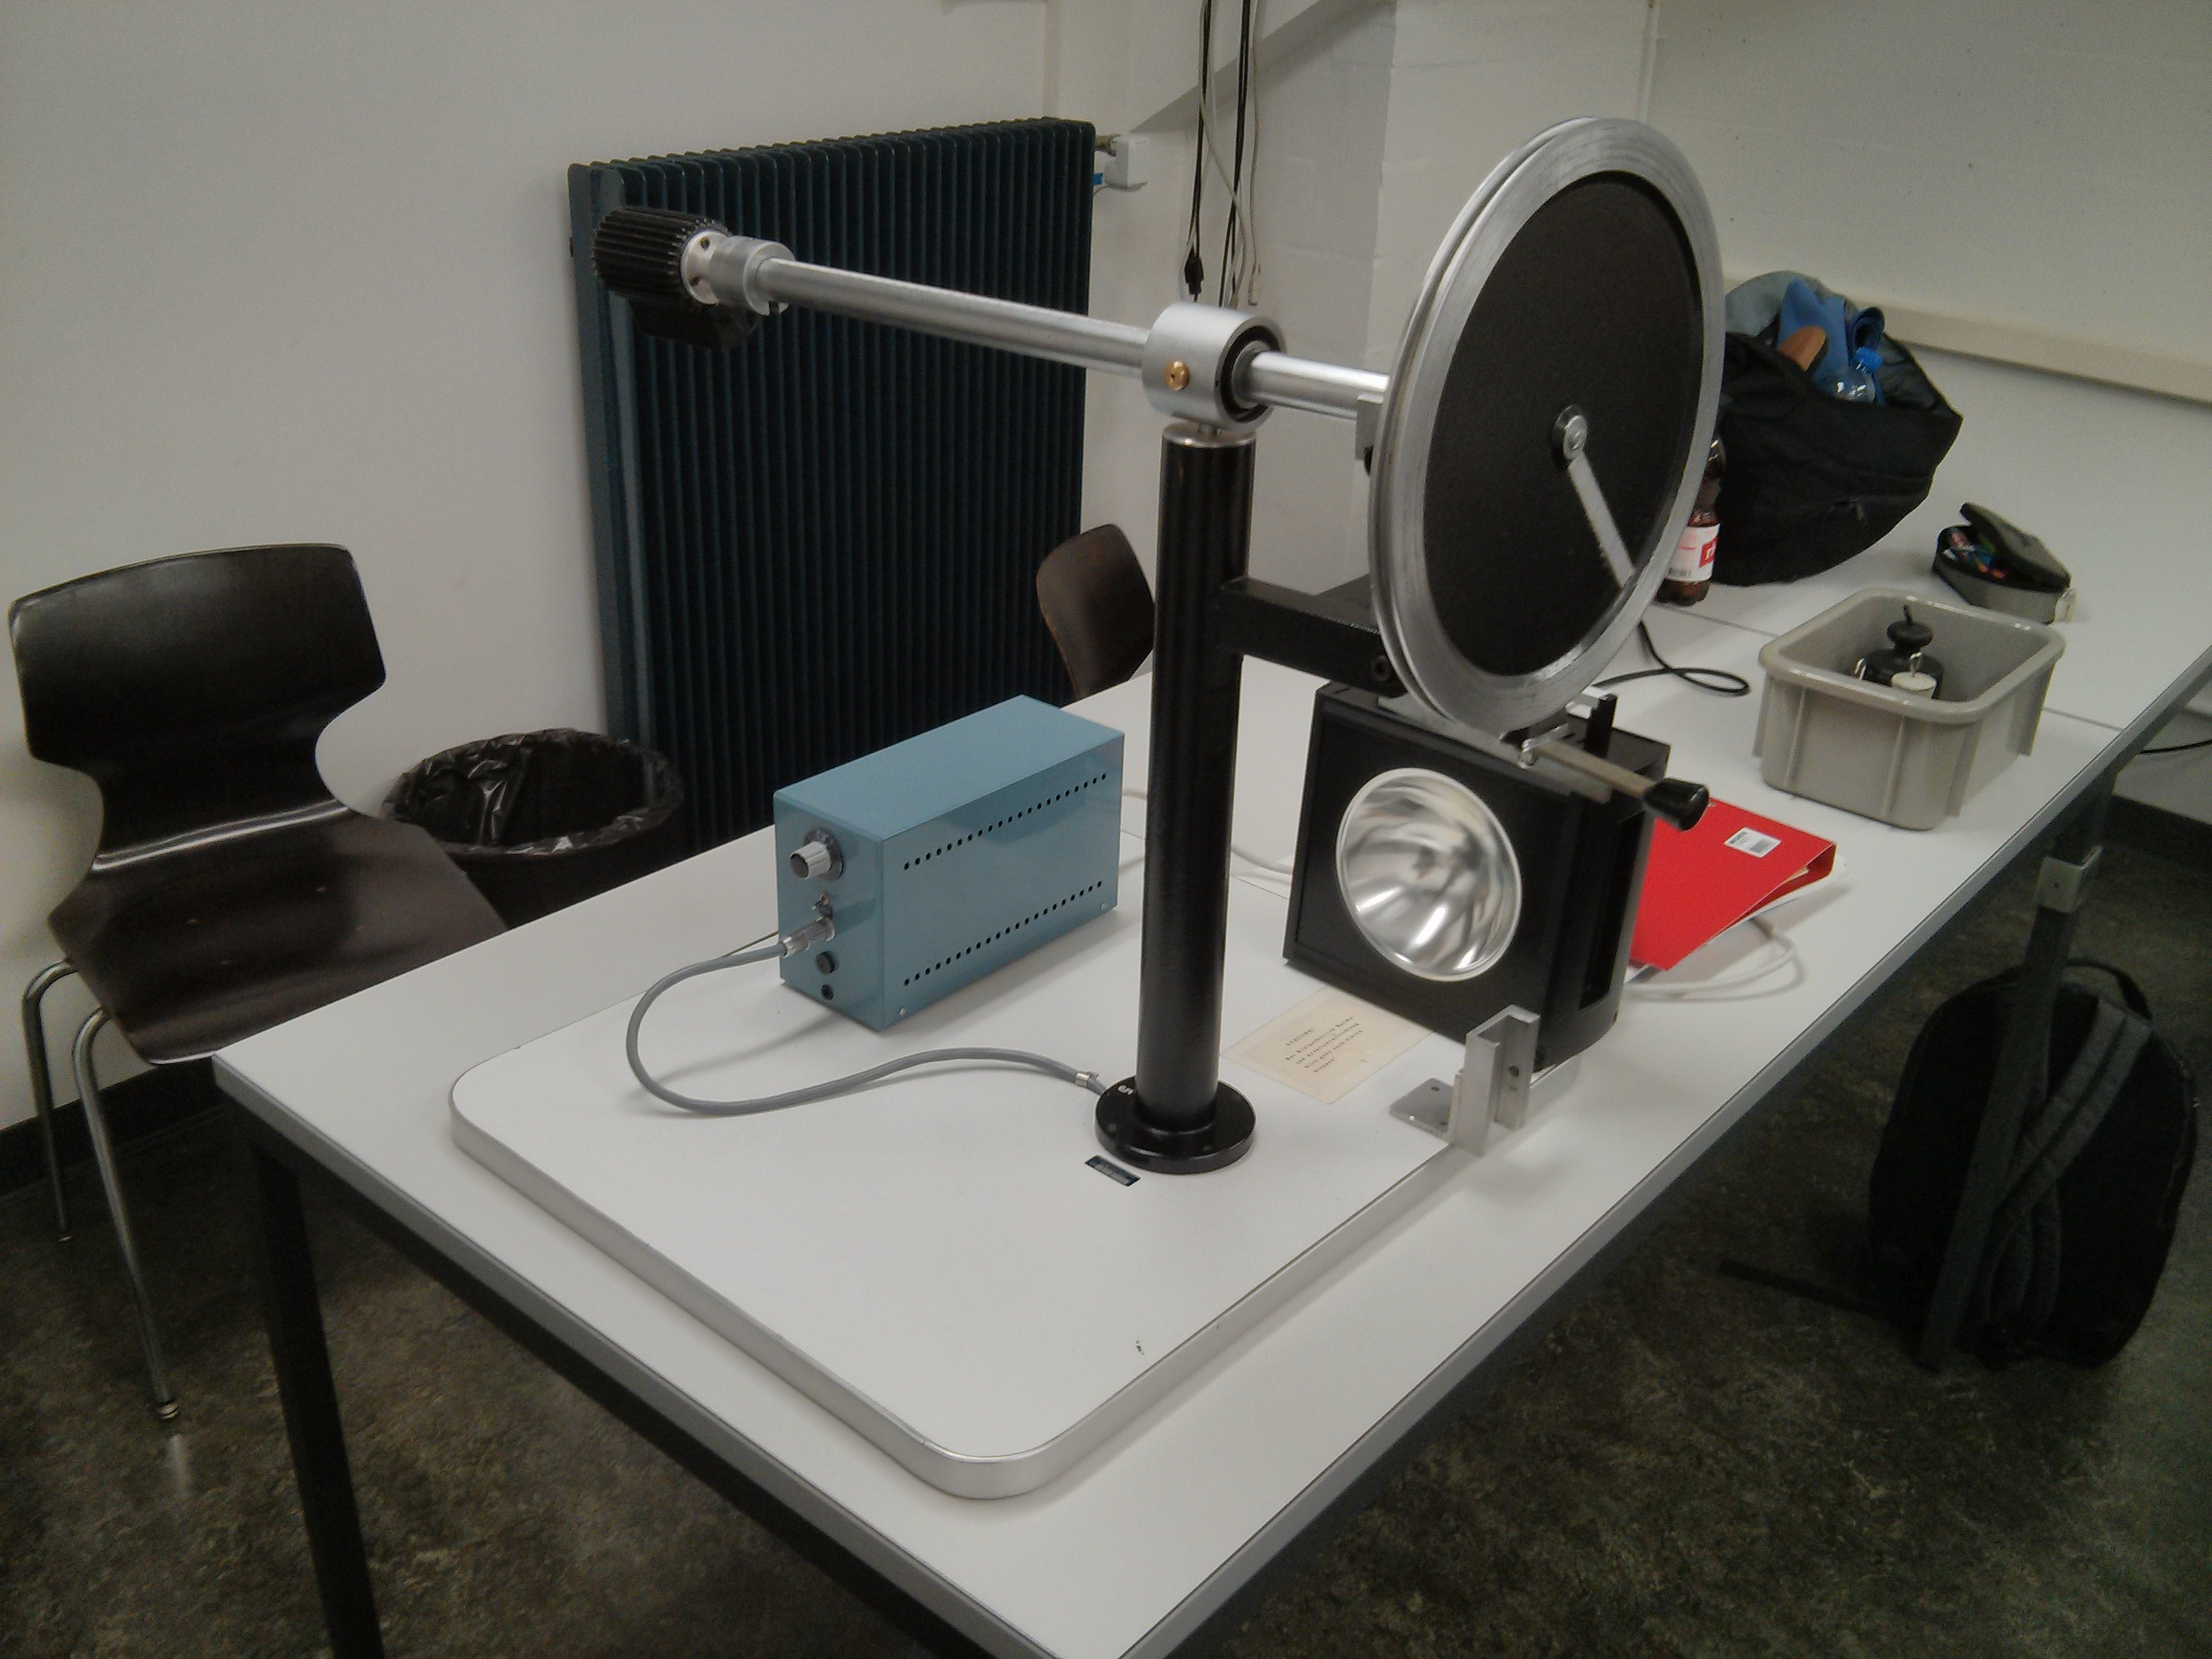
\includegraphics[width=0.9\textwidth]{img/assembly.jpg}
	\caption{Experiment Assembly}
	\label{fig:assembly}
\end{figure}


\section{Measurements}
\subsection{moment of inertia}
\begin{figure}[H]
	\centering
  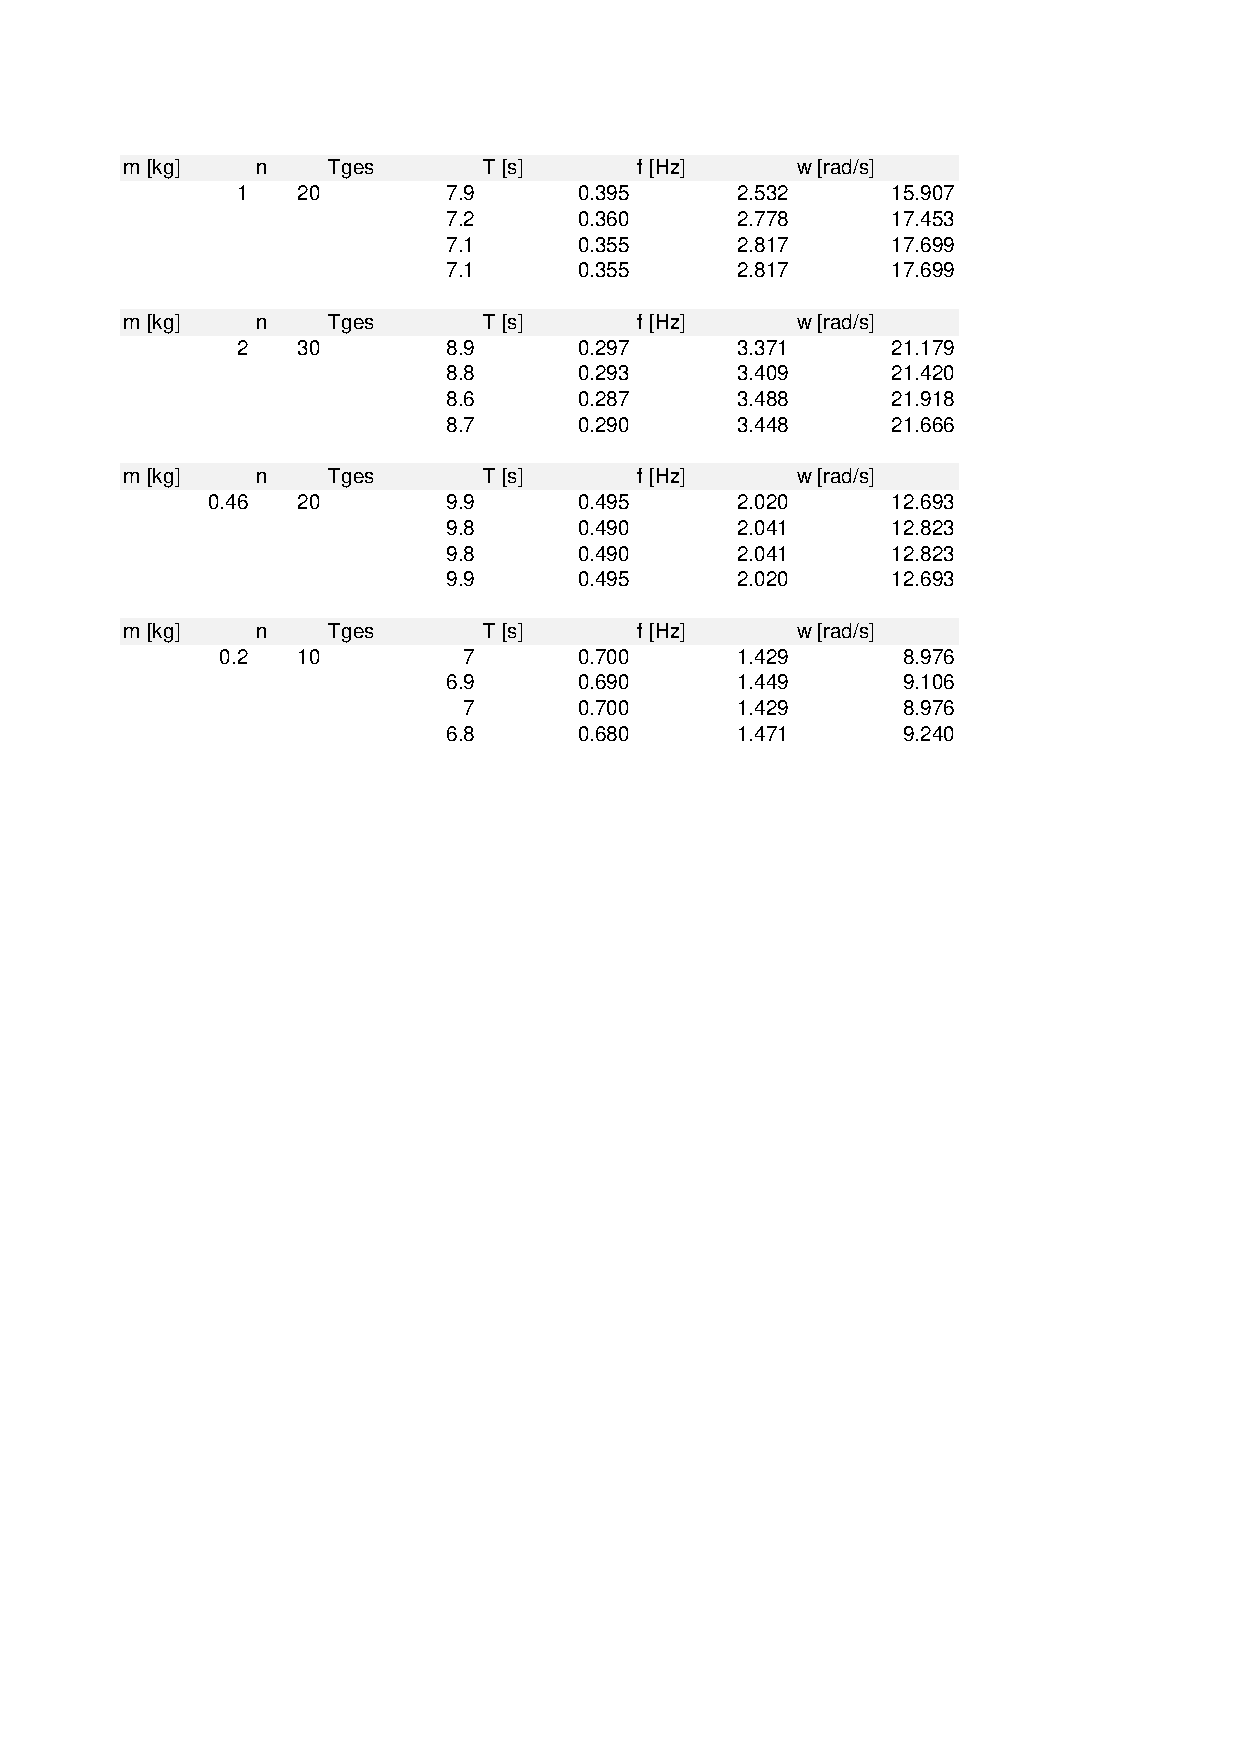
\includegraphics[width=0.9\textwidth]{diag/inertia.pdf}
	\caption{Measured moments of inertia}
	\label{fig:inertia}
\end{figure}

\subsection{Precession}
\begin{figure}[H]
	\centering
  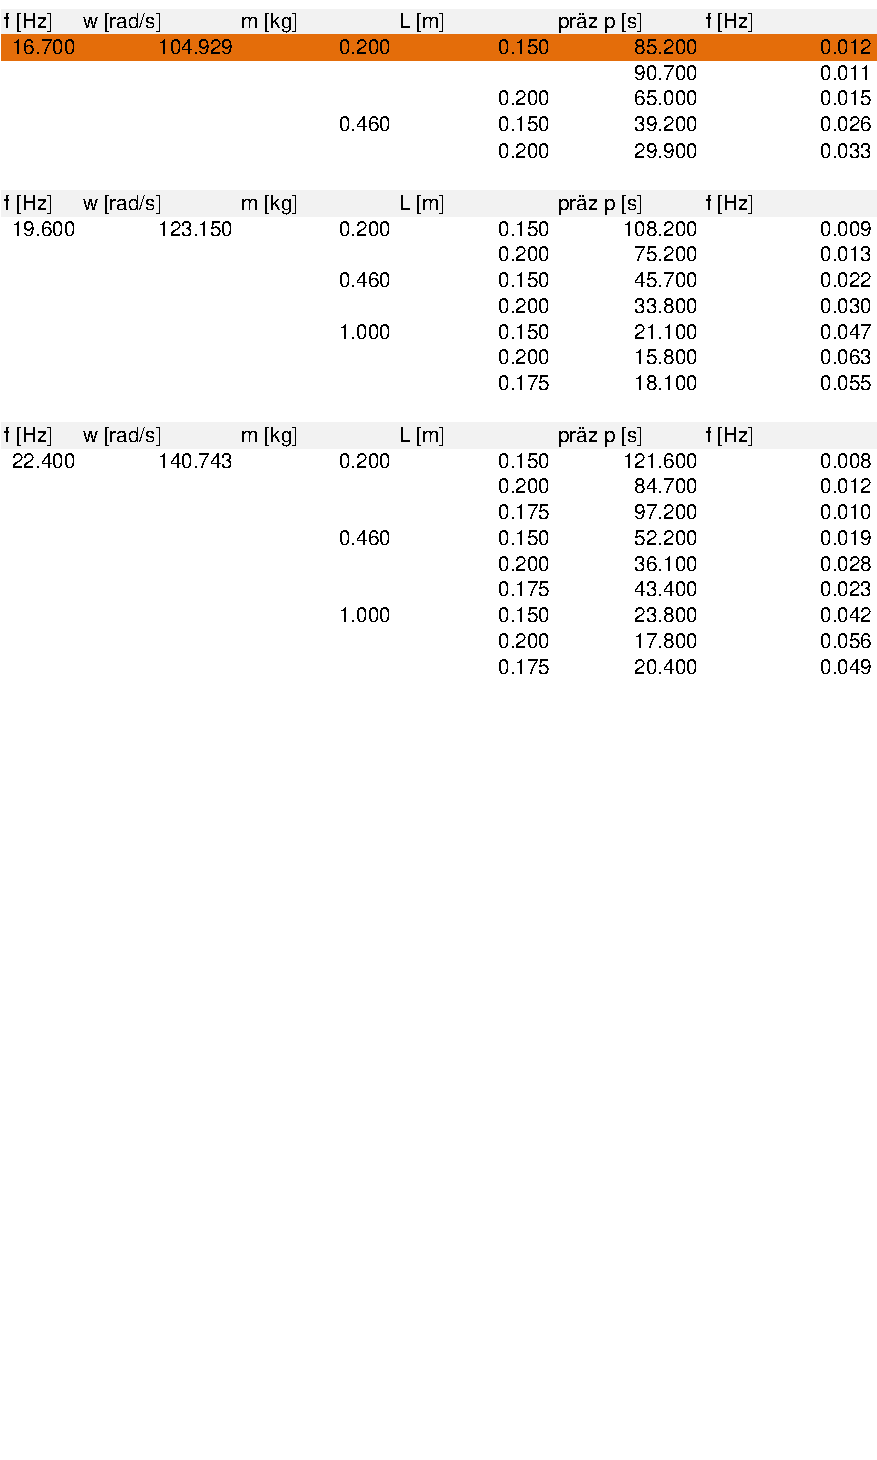
\includegraphics[width=0.9\textwidth]{diag/precession.pdf}
	\caption{Measured precession frequencies (the value highlighted in red was dismissed due to clearly visible impact of friction}
	\label{fig:precession}
\end{figure}

\section{Analysis and Discussion}

\subsection{Moment of inertia $J$}
To calculate the moment of inertia $J$ of the spinning disk, we use formula \ref{eq:inertia} and our measured values for $\omega_0$:

\begin{table}[H]
\centering
\begin{tabular}{|l|cccc|}
\hline
$h = 1\unit{m}$ & $ m = 0.2 \unit{kg}$ & $m = 0.46 \unit{kg}$ & $m = 1 \unit{kg}$ & $m = 2 \unit{kg}$\\
\hline\hline
$\omega_0$ [$\unit{rad/s}$] & $9.075 \pm 0.0631$ & $12.758 \pm 0.0374$ & $17.190 \pm 0.432$ & $21.546 \pm 0.159$\\ \hline
$J$ [$\unit{kg\cdot m^2}$] & $0.0440 \pm 0.00331$  & $0.0471 \pm 0.00072$ & $0.0482 \pm 0.0033$ & $0.0481 \pm 0.00334$ \\ \hline
\end{tabular}
\label{tab:inertia_results}
\caption{The resulting momenta of inertia $J$ for different values of $m$}
\end{table}

To calculate the effective moment of inertia $J$, we average all the momenta of inertia above, which yields

\begin{equation}
J = (0.0468	 \pm 0.000974) \unit{kg\cdot m^2}
\end{equation}

\subsection{Precession Period $T_P$}
\subsection{Sources of error}

\section{Conclusion}

\begin{thebibliography}{9}

\bibitem{physcript13}
  Peter Wurz,
  \emph{Anleitung zum Physikpraktikum}
  FS2013

\end{thebibliography}

\end{document}
